\documentclass{article}
\author{}
\usepackage{caption}
\usepackage{subcaption}
\usepackage{graphicx} %I need to include some graphs in this document
\usepackage{amsmath}
\usepackage[margin=1.2in]{geometry}

\begin{document}
\paragraph*{}
\begin{itemize}
\item \mbox{08/09}
\begin{align*}
&T^*=k_BT/\epsilon \\
&\rho^*=\rho\sigma^3\\
&\kappa^*=\kappa\sigma^2\sqrt{m}/(k_B\sqrt{\epsilon})\\
&t^*=t\sqrt{\epsilon}/(\sigma\sqrt{m})
\end{align*}
\item \mbox{08/20}
\begin{align*}
\vec{w}^2&=(\alpha\vec{r}+\beta\vec{b})^2 \\
&=\alpha^2r^2+\beta^2b^2+2\alpha\beta\vec{r}\cdot\vec{b}\\
&=\alpha^2r^2+(1-\alpha\frac{\vec{r}\cdot\vec{b}}{b^2})^2b^2+2\alpha(1-\alpha\frac{\vec{r}\cdot\vec{b}}{b^2})\vec{r}\cdot\vec{b}\\
&=\alpha^2r^2+(1+\alpha^2\frac{(\vec{r}\cdot\vec{b})^2}{b^4}-2\alpha\frac{\vec{r}\cdot\vec{b}}{b^2})b^2+2\alpha(1-\alpha\frac{\vec{r}\cdot\vec{b}}{b^2})\vec{r}\cdot\vec{b}\\
&=\alpha^2r^2+b^2-\alpha^2\frac{(\vec{r}\cdot\vec{b})^2}{b^2}\\
&=b^2+\frac{\vert\alpha\vert^2}{b^2}(r^2b^2-(\vec{r}\cdot\vec{b})^2)
\end{align*}
\item 08/26
\paragraph*{}
In our calculations, the standard deviation of temperature in a certain slab $m$ is expressed as
\begin{equation}
\sigma_{m,s}=\sqrt{\frac{\sum\limits_{i=1}^\mathcal{N}\left( T_{m,i}-\overline{T}_m\right)}{\mathcal{N}-1}}
\end{equation}
where $\overline{T}_m$ is the average value for measurements $T_{m,i}$ and $\mathcal{N}$ represents the total number of measurements.The standard deviation of the averaged value $\overline{T}_m$, therefore, is given by
\begin{align}
\sigma_m &=\frac{\sigma_{m,s}}{\sqrt{\mathcal{N}}}\\
&=\sqrt{\frac{\sum\limits_{i=1}^\mathcal{N}\left( T_{m,i}-\overline{T}_m\right)}{\mathcal{N}(\mathcal{N}-1)}}
\end{align}
\paragraph*{}
With a set of data $(\overline{T}_m,\sigma_m)$ where $m$ goes from 0 to N-1 in our model, we do the fit to the cosine function to determine and fitting parameter of amplitude, which is $\Delta T$ in Eq.(1). The standard deviation of $\Delta T$ is determined at the same time.Then by using Eq.(2) we can get a relation between $\sigma_{\Delta T}$ and $\sigma_{\kappa_{\mbox{eff}}}$, which is
\begin{equation}
\frac{\sigma_{\kappa}}{\kappa_{\mbox{eff}}}=\frac{\sigma_{\Delta T}}{\Delta T}
\end{equation}
Thus $\sigma_{\kappa_{\mbox{eff}}}=\kappa_{\mbox{eff}}\sigma_{\Delta{T}}/\Delta{T}$ gives the standard deviation of $\kappa$.
\end{itemize}

\section*{Liquid}
\begin{itemize}
\item \mbox{08/09}\\
Cutoff distance for LJ potential 3.0$\sigma$\\
Width of slab $d=a=5.31\AA$, 1.56 in reduced units with LJ constant $\sigma$ for Argon 3.405$\AA$ 
The simulations are conducted on supoercells of $6\times6\times{N}$ cubic conventional cells with $N$ a parameter for approching the bulk limit. This 6 by 6 simulation proves reasonable from comparing the behaviour of $\kappa(q)$ around the $q=0$ with that predicted by Debye Model and in order to do this, we treated the solution of Boltzmann equation in two different ways.
\item \mbox{08/09}\\
Time \\
The LJ unit, a unit time for Argon should be $\tau_{LJ}$=2.16ps\\
For short sample time step is $\Delta t^*=6.965\times10^{-3}$,while for longer sample $\Delta t^*=2\times6.965\times10^{-3}$\\
\item \mbox{08/11}\\

\begin{equation*}
%\centering
X = [\delta-(v_H^2-v_C^2)]\cdot\frac{\delta}{\lvert \vec{v}_H+\vec{v}_C\lvert^2}\cdot\frac{b^2}{b^2r^2-(\vec{b}\cdot\vec{r})^2}
\end{equation*}
For safety in evolutions, we'd better keep $X$ negative. As shown in Eqs.(10) the last two terms are positive so $\delta-(v_H^2-v_C^2)=2\Delta/m-(v_H^2-v_C^2)$ dominates. It is found in tests that $v_H^2-v_C^2$ sometimes touches the ground of 3(in L-J reduced units), so if $W$ were set to be 480 in this case, for instance, we would soon find errors in the data. One may insist on a $W$ which is much smaller than 60 to enable inputs with larger amplitudes for the simple reason that large imposes converge much faster. However, this proves unnecessary: it has been shown in Muller-Plathe's method that validity of linear response theory breaks down for large variation with $W=15$, which is parallel to the impose with  $\dot{e}=10.120$ in our theory. So even if, with lower $W$ and larger input amplitude, there is nothing wrong with the calculation of vector $\vec{w}$, it is meaningless to do calculations of this kind without the validity of linear response theory. It is been tested that $W=60$ does not work for $\dot{e}=10.120$, therefore, our choice of $W$ seems quite reasonable.
\item \mbox{08/11}\\
Time step$\Delta t^*=6.965\times10^{-3}$ and it is very interesting that this is a guess from dimension argument.\\
We choose crystal constant a as the width of the slab so we can keep 144 atoms in each slab. By doing this, we can ensure a quite large $(v_H^2-v_C^2)$
\item \mbox{08/23}\\

\paragraph*{}
Here, the critical parameter for the MullerPlathe is W=120 while for the new algorithm is e=1.265, and to ensure a solution for X, W is chosen to be 60.
\item {08/26}
\begin{figure}[h]
    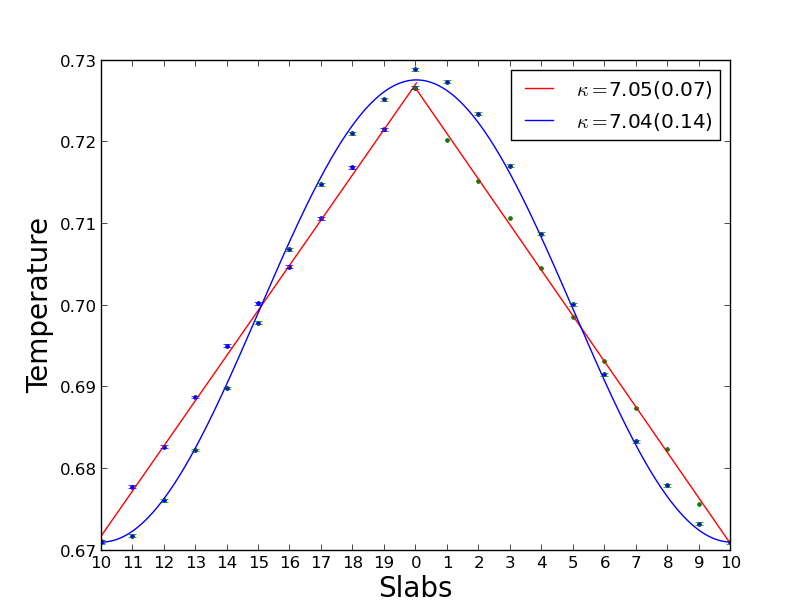
\includegraphics[height=6cm]{amplitude1.png}
\end{figure}
\end{itemize}

\section*{Crystal}
\begin{itemize}

\item \mbox{08/11}
In experiment, 
\begin{align*}
\kappa^*=\kappa\times 52.943
\end{align*}
for crystal, $\kappa=0.31 W/(m\cdot K), \kappa^*=16.41------- 77K$\\
for liquid, $\kappa=0.1324 W/(m\cdot K), \kappa^*=7.01------- 85K$\\
CRC Handbook of Chemistry and Physics,85th Edition,	David R. Lide (Editor) ,CRC Press
\item \mbox{08/11}\\
\begin{figure}[h]
    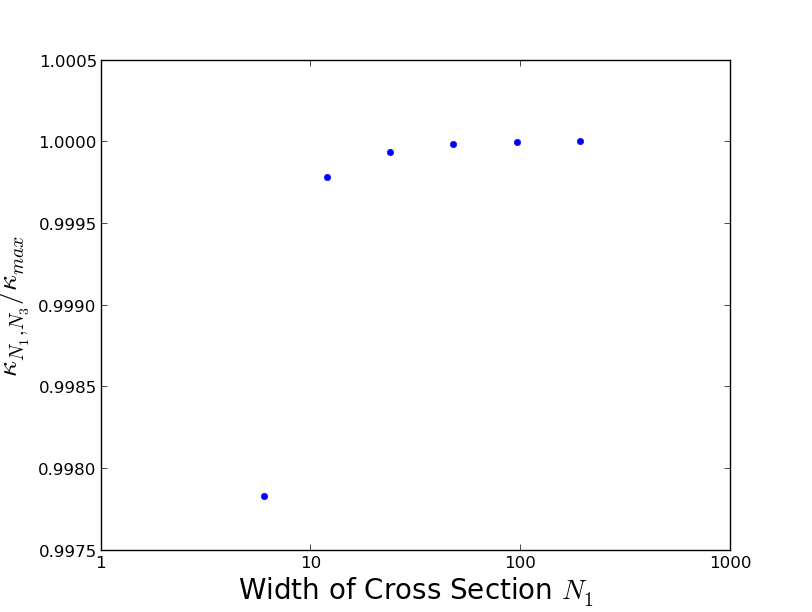
\includegraphics[height=6cm]{Cross5.png}
\end{figure}
I changed the x axis so this figure is more reader-friendly.

\item {08/23}\\
  The temperature for simulation on crystal 1s 80 K, which is 0.66 in LJ unit and the amplitude of the sine function in temperature profile is 0.03 in LJ unit.  
\item {08/23}\\
  N3 is 12,16,20,28,32,36,56,64,72,120,128,136 in my simulation.
  \item \mbox{08/23}\\
\begin{figure*}[h]
    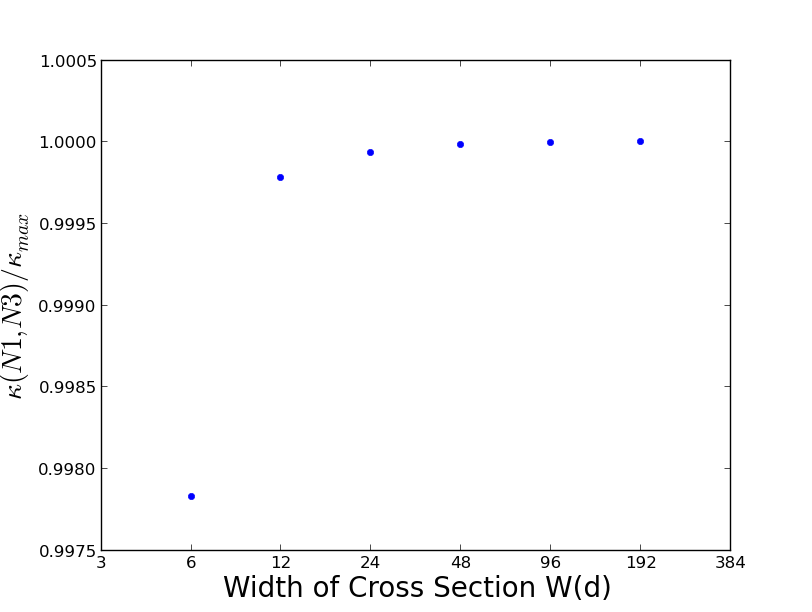
\includegraphics[height=6cm]{Cross3.png}
\end{figure*}
summing over Brillouin Zone, the length of the sample is 500a=500d, the ratio is devided by the kappa(192)
\end{itemize}
\paragraph*{}
\section*{Extrapolation}
\begin{itemize}
\item \mbox{08/09}\\
Temperature approximately 80K, 0.66 in LJ unit, with the scaling $\epsilon/k_B=119.6K$, I keep the temperature variance 0.03 during the simulation(LJ unit) to keep my system efficient.We run those systems at constant temperature.
\item \mbox{08/11}\\
\begin{equation*}
\frac{\kappa(q)}{\kappa_D}=\frac{3-p}{N}\cos^2(qd/2)\sum\limits_{\vec{Q}} \frac{Q_x^2}{\vec{Q}^2}  (\frac{Q_D}{Q})^p\cdot F(q,u)
\end{equation*}
$Q_D=(6\pi^2(N/V))^{1/3}$ in the case of fcc $Q_D=(3/\pi)^{1/3}\frac{2\pi}{a}=0.985\frac{2\pi}{a}$\\
$Q_x$ is the projection of $\vec{Q}$ in (1,1,$\bar{1}$) direction.

\end{itemize}
\end{document}